\section{谱划分方法的比较}
\label{sec:graph-spectral-partition-comparison}

RatioCut与NCut同属基于拉普拉斯二次型松弛的谱划分方法，两者的算法骨架高度一致，核心区别仅在于\emph{如何定义子图的规模}：RatioCut按“顶点个数$|A|$”计规模，追求两侧节点数量的均衡；NCut按“度数总和（体积$\operatorname{vol}(A)$）”计规模，衡量跨割权相对于两侧总度数的比例。表~\ref{tab:ratiocut-vs-ncut}汇总了两种方法在各个环节的一一对应关系。

\begin{table}[!htb]
\centering
\caption{RatioCut与NCut谱划分方法的核心要素对比。}
\label{tab:ratiocut-vs-ncut}
\footnotesize
\begin{tabular}{lll}
\toprule
对比维度 & RatioCut（比例割） & NCut（归一化割）\\
\midrule
均衡目标 & 节点个数$|A|,|B|$均衡 & 度体积$\operatorname{vol}(A),\operatorname{vol}(B)$均衡\\
目标函数 & $c(A,B)\bigl(\frac{1}{|A|}+\frac{1}{|B|}\bigr)$ & $c(A,B)\bigl(\frac{1}{\operatorname{vol}(A)}+\frac{1}{\operatorname{vol}(B)}\bigr)$\\
两值向量$f_i$ & $\sqrt{|B|/|A|},-\sqrt{|A|/|B|}$ & 式~\eqref{eq:ncut-indicator-vector}的两值\\
等价Rayleigh商 & $\dfrac{\bm f^\top\bm L\bm f}{\bm f^\top\bm f}$ & $\dfrac{\bm f^\top\bm L\bm f}{\bm f^\top\bm D\bm f}$\\
松弛算子 & 组合拉普拉斯$\bm L=\bm D-\bm W$ & 对称归一化$\mathcal L=\bm D^{-1/2}\bm L\bm D^{-1/2}$\\
下界与排序 & $\lambda_2(\bm L)$，按$\bm v_2$排序 & $\mu_2(\mathcal L)$，按$\bm f=\bm D^{-1/2}\bm z_2$排序\\
Cheeger保证 & 需另行给出相应尺度的界 & $\operatorname{NCut}(S_N)\leq 2\sqrt{2\operatorname{OPT}_N}$\\
\bottomrule
\end{tabular}
\end{table}

在正则图上，两种目标成比例；度数不完全相同时，即使差异较小，也不能保证最优划分一致。下面通过一个具体的四点加权路径算例直观展示这一分歧。

\paragraph{加权路径上的最优割分歧}

考虑图~\ref{fig:graph-partition-weighted-path}所示的四顶点路径$1\!-\!2\!-\!3\!-\!4$，将其三条边的权重设为中间重、两端轻：$w_{12}=1$，$w_{23}=2$，$w_{34}=1$。由此算出四个顶点的加权度依次为$d_1=1,d_2=3,d_3=3,d_4=1$，全图总体积为$\operatorname{vol}(V)=8$。

\begin{BookInlineFigure}
  \centering
  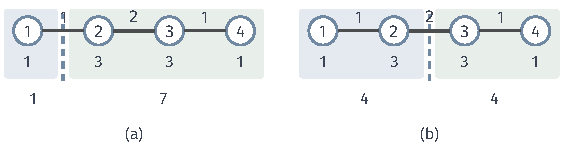
\includegraphics{figures/03-graphs/05-matrices-and-spectra/tikz/partition-weighted-path/figure.pdf}
  \caption{加权路径（边权$1,2,1$）上的两个关键候选割。(a) 切下左端点$1$：只切断权重为$1$的端边，两侧顶点数为$1$对$3$，两侧体积为$1$对$7$。(b) 沿中间边切开：需切断权重为$2$的粗边，但两侧顶点数（$2$对$2$）与体积（$4$对$4$）均相等。顶点下方标注加权度。}
  \label{fig:graph-partition-weighted-path}
\end{BookInlineFigure}

我们重点比较图~\ref{fig:graph-partition-weighted-path}标出的两种切法：
\begin{enumerate}
\item \emph{候选一：切下低度端点$\{1\}\mid\{2,3,4\}$}（图a，与切下右端点$\{4\}\mid\{1,2,3\}$对称）。这一刀避开了中间权重为$2$的粗边，只切断权重为$1$的轻边$12$，故割权$c=1$。两侧的节点个数为$|A|=1,|B|=3$，而两侧的体积则悬殊为$\operatorname{vol}(A)=1,\operatorname{vol}(B)=7$。代入两个目标函数：
\[
\begin{aligned}
  \operatorname{RatioCut}(\{1\}) &= 1\times\left(\frac{1}{1}+\frac{1}{3}\right) = \frac{4}{3}\approx 1.333, \\
  \operatorname{NCut}(\{1\}) &= 1\times\left(\frac{1}{1}+\frac{1}{7}\right) = \frac{8}{7}\approx 1.143.
\end{aligned}
\]
\item \emph{候选二：切断中间重边$\{1,2\}\mid\{3,4\}$}（图b）。这一刀直接切断权重为$2$的中间边$23$，割权升至$c=2$，但换来了两侧规模相等——两侧节点个数为$2$对$2$，两侧体积均为$1+3=4$。代入两个目标函数：
\[
  \operatorname{RatioCut}(\{1,2\}) = 2\times\left(\frac{1}{2}+\frac{1}{2}\right) = 2,
  \qquad
  \operatorname{NCut}(\{1,2\}) = 2\times\left(\frac{1}{4}+\frac{1}{4}\right) = 1.
\]
\end{enumerate}

至于其余非空二分（如将两端点合为一组的$\{1,4\}\mid\{2,3\}$，或奇偶交错的$\{1,3\}\mid\{2,4\}$），它们同时切断了两条或三条边，割权不低于$2$且规模不比中间割更优。图~\ref{fig:graph-comparison-four-bipartitions}与下表展示了四类代表性二分；下表还列出了切下内部顶点的第五类，从而覆盖所有非空二分（对称情形合并）的结构与指标：

\begin{BookInlineFigure}
  \centering
  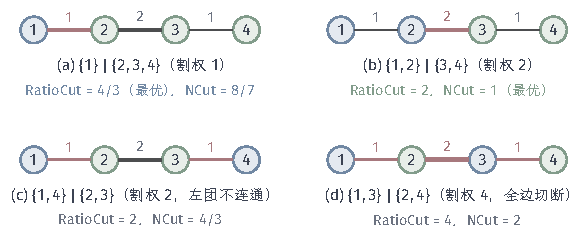
\includegraphics[width=98.316mm]{figures/03-graphs/05-matrices-and-spectra/tikz/comparison-four-bipartitions/figure.pdf}
  \caption{加权路径（边权$1,2,1$）的四类非空二分结构对比。蓝色与绿色区分两侧子集，红色边表示被切断的跨割边。(a) 切下单个端点，RatioCut达到全局最小$4/3$；(b) 切断中间重边，NCut达到全局最小$1$；(c) 两端点合并为一侧，同时切断两条端边且左侧不连通；(d) 奇偶交错分组，三条边全部被切断。}
  \label{fig:graph-comparison-four-bipartitions}
\end{BookInlineFigure}
\begin{center}
\small
\setlength{\tabcolsep}{4pt}
\begin{tabular}{lccccc}
\toprule
候选划分 & 割权$c$ & 节点数 & 两侧体积 & RatioCut & NCut\\
\midrule
$\{1\}\mid\{2,3,4\}$ & $1$ & $1,3$ & $1,7$ & $\mathbf{4/3}$ & $8/7$\\
$\{1,2\}\mid\{3,4\}$ & $2$ & $2,2$ & $4,4$ & $2$ & $\mathbf{1}$\\
$\{2\}\mid\{1,3,4\}$ & $3$ & $1,3$ & $3,5$ & $4$ & $8/5$\\
$\{1,4\}\mid\{2,3\}$ & $2$ & $2,2$ & $2,6$ & $2$ & $4/3$\\
$\{1,3\}\mid\{2,4\}$ & $4$ & $2,2$ & $4,4$ & $4$ & $2$\\
\bottomrule
\end{tabular}
\end{center}

枚举全部二分后，RatioCut的最小值为$4/3$，由两种端点割取得；NCut的最小值为$1$，由中间割取得。端点割将割权从$2$减为$1$，足以抵消RatioCut中的顶点数失衡代价；在NCut中，端点仅占总体积的$1/8$，其代价$8/7$仍大于中间割的$1$。这一差异来自两个目标采用的规模度量。

\paragraph{正则图上的统一性与实践选择建议}

当图是加权度恒为常数$d>0$的$d$正则图时，任意子集$A$的体积恒等于节点数的$d$倍：$\operatorname{vol}(A)=d|A|$。此时NCut与RatioCut严格成正比：
\[
\operatorname{NCut}(A,B)
=c(A,B)\left(\frac{1}{d|A|}+\frac{1}{d|B|}\right)
=\frac{1}{d}\operatorname{RatioCut}(A,B),
\]
对称归一化拉普拉斯也简化为$\mathcal L=\frac{1}{d}\bm L$，两种离散目标具有相同的最优划分。若选择相同的特征方向并使用一致的并列处理规则，谱扫描的排序与结果也相同；重特征值或多个最优切口可能使不同实现返回不同划分。

选择目标应依据任务如何衡量规模。若每个顶点代表等量负载，可以考虑RatioCut；若关心每侧跨组连接占总连接量的比例，可以考虑NCut。二者都是软性的均衡目标，均不保证指定的组大小或内部密度。若任务要求严格等分，应另加规模约束，并重新分析算法和保证。
